\scanpage{156}
% archive foliation: 155

\deleted{\unsure{5}}\inserted{$B_1$})
$\deleted{\unsure{S}}\ \mathrm{Car}(S)\simeq\mathrm{Car}(S^*)$

\figure{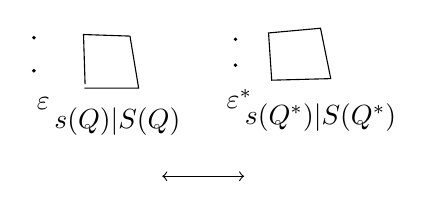
\begin{tikzpicture}[x=1cm,y=1cm]
\draw (0.65,0.55) -- (0.63,1.18) -- (1.22,1.16) -- (1.33,0.50) -- (0.64,0.50);
\fill (0,1.14) circle (0.025);\fill (0,0.72) circle (0.025);
\node at (0.12,0.30) {$\varepsilon$};
\node at (1.06,0.08) {$\unsure{s(Q)|S(Q)}$};
\draw (3.02,0.60) -- (2.98,1.20) -- (3.64,1.26) -- (3.77,0.62) -- cycle;
\fill (2.56,1.12) circle (0.025);\fill (2.56,0.79) circle (0.025);
\node at (2.61,0.36) {$\varepsilon^*$};
\node at (3.64,0.12) {$\unsure{s(Q^*)|S(Q^*)}$};
\draw[<->] (1.63,-0.62) -- (2.67,-0.62);
\end{tikzpicture}}

\margin{expliciter utilisant
\[
\left\{\begin{array}{l}
\varepsilon\wedge\varepsilon^*\wedge\omega(Q)=1\\
\omega(Q)\simeq\omega(Q^*)\\
Q^*\simeq\varepsilon\wedge Q\ ;\quad Q\simeq\varepsilon^*\wedge Q^*
\end{array}\right.
\]}

$C_1$) Relation avec la donnée d'un
\deleted{espace} plan affine $\unsure{V}$ sur $\mathbb F_3$
et de \deleted{$\unsure{\operatorname{card}P(V)}=4$},
$\operatorname{Card}(\unsure{E}=P(V))=4$, \deleted{Aut}
\[
\unsure{\mathfrak G|\mathfrak S}_{P(V)}\simeq
\underline{\operatorname{Aut}}(V)(\mathbb F_3)\simeq
\mathrm{GP}(\unsure{1|2},\mathbb F_3)
\]
et une partition \inserted{$(2,2)$ de $E$ (en \unsure{antipodismes})}

i.e. \unsure{Structure carrée} sur $E$.
\[
\operatorname{card}(E_i)=3\qquad i\in E
\]
\diagram{\begin{tikzcd}
E_i\times E_j & V\arrow[l,"\sim"'] &
\text{pour }i,j\in E\quad i\neq j
\end{tikzcd}}

\margin{\diagram{\begin{tikzcd}V\arrow[r,"p_i"']&E_i\end{tikzcd}}
$V\subset\prod E_i$}

\figure{\begin{tikzpicture}[x=1cm,y=1cm]
\fill (0.10,1.70) circle(0.025);\fill(0.25,2.03) circle(0.025);\fill(0.48,2.37) circle(0.025);
\fill (1.35,2.50) circle(0.025);\fill(1.77,2.44) circle(0.025);\fill(2.23,2.27) circle(0.025);
\fill (2.80,1.57) circle(0.025);\fill(2.71,1.17) circle(0.025);\fill(2.66,0.86) circle(0.025);
\fill (0.62,0.51) circle(0.025);\fill(1.04,0.36) circle(0.025);\fill(1.46,0.31) circle(0.025);
\fill(5.34,1.06) circle(0.025);\fill(5.56,1.07) circle(0.025);\fill(5.79,1.08) circle(0.025);\fill(6.00,1.09) circle(0.025);
\draw(5.22,1.01)..controls(5.30,0.91)and(5.40,0.97)..(6.26,1.00);
\end{tikzpicture}}

Groupe d'automorphismes \unsure{trilitaire}
d'ordre $3^3\times2^4=3.144$ \unsure{,}

Opère sur $\unsure{\mathfrak G|\mathfrak S}_{\varepsilon}$
\margin{$\varepsilon=\coprod_{i\in E}E_i$}

et laisse invariant \deleted{trois} un syst.
de $3$ sous-groupes $G_\alpha$
($\alpha\in\deleted{\unsure{\mathcal E}}\mathrm{Car}(E)=\mathrm{Antip.}(E)$)
Le stabilisateur d'un $G_\alpha$ est le groupe des
automorphismes d'une bi-ditriade. Opère
fidèlement sur $G_\alpha$, sous groupe d'ordre $\unsure{10|16}$ de
$\operatorname{Aut}(G_\alpha)$
\inserted{(d'ordre $\unsure{2.(8!)|2.(6!)}$)}

\margin{les $G_\alpha$ ont un
$3$-sous-groupe de Sylow \inserted{$V_0$} en commun, et
\deleted{\unsure{qui est}} \unsure{d'indice} \illegible{2}
\deleted{la \unsure{décomposition} \illegible{2} de $V$}
\deleted{et $\unsure{V/V_0|G/V_0}$ est le groupe du
\unsure{carré} \illegible{2}}
$N_{\unsure{\operatorname{Aut}G_\alpha}}(V_0)/V_0$
\unsure{opère} \illegible{2}
(groupe du carré)}
